\chapter{Método de triangulación}

Mediante este método se determinan las coordenadas $(x,y,z)$ de un punto utilizando la posición bidimensional dada por las perspectivas de dos proyecciones de las que se conocen los centros de perspectiva y planos de proyección \cite{PresUnivYonsei}.

Escena con dos dimensiones:

\begin{figure}[H]
  \centering
    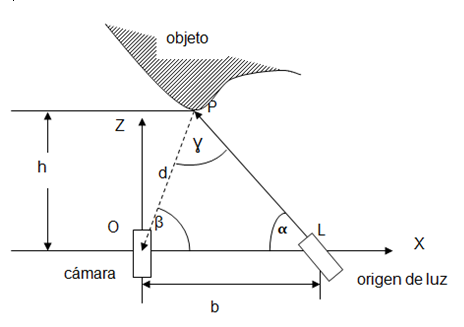
\includegraphics[width=0.65\textwidth]{./Cap2_videomapping/triangulacion.PNG}
  \caption{Propiedades trigonométricas para escena bidimensional.}%Geometía de Cámaras  StereoReview pag 154. fig 6.1%
  \label{fig:Triangulacion}
\end{figure}

Este método tiene como objetivo calcular la distancia $d$ de la cámara al punto $P$ a partir de los ángulos $\alpha$, $\beta$ y la distancia $b$ entre el proyector y la cámara.
El ángulo $\alpha$ y la distancia $b$ son dados por la configuración de la escena.
El ángulo $\beta$ está dado por la geometría de la proyección.

\[
\left.
\begin{array}{l}
\frac{d}{\sin (\alpha)} = \frac{b}{\sin (\gamma)} 	\\
\gamma = \pi - (\alpha + \beta)						\\
\sin (\pi - \gamma) = \sin (\gamma)
\end{array}
\right \rbrace
\frac{d}{\sin(\alpha)} = \frac{b}{\sin(\pi - \gamma)} = \frac{b}{\sin(\alpha + \beta)} \Rightarrow d = b . \frac{\sin(\alpha)}{\sin(\alpha + \beta)}
\]

Las coordenadas cartesianas quedan determinadas por:
\[
X_0 = d. \cos (\beta)
\]
\[
Z_0 = d. \sin (\beta) = h
\]

Escena con tres dimensiones:

\begin{figure}[H]
  \centering
    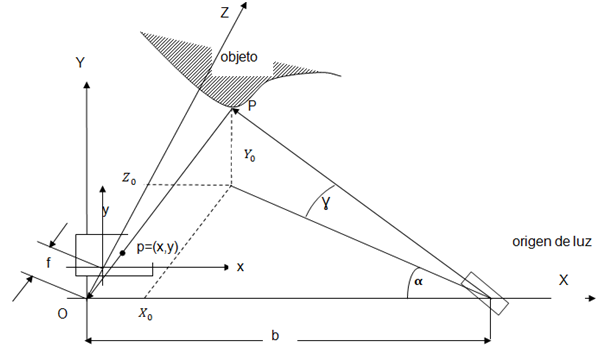
\includegraphics[width=0.65\textwidth]{./Cap2_videomapping/triangulacion-2.PNG}
  \caption{Propiedades trigonométricas para escena tridimensional.}
  \label{fig:Triangulacion2}
\end{figure}

Se asume $Z = f$ siendo $f$ el plano en el cuál se proyecta el punto $P(X_0, Y_0, Z_0)$, obteniendo como resultado de la proyección el punto $p(x,y)$.
El centro óptico del proyector está situado en el eje $X$.
Se considera realizada una pre-calibración en la cual se define:
\[
P = (x,y), \quad \frac{X_0}{x} = \frac{Z_0}{f} = \frac{Y_0}{y} = k \to (k * x,k * y,k * f)
\]
Por trigonometría:
\[
\tan (\alpha) = \frac{Z_0}{(b - X_0)} \Rightarrow Z_0 = \tan (\alpha) (b - X_0) \quad 
\]
\[
k * f = \tan (\alpha)(b - k * x)
\]
\[
k (f + x * \tan (\alpha)) = b * \tan (\alpha)
\]
\[
k = \frac	{b * \tan (\alpha)}{f + x * \tan (\alpha)}
\]
\[
X_0 = \frac{x * b * \tan (\alpha)}{f + x * \tan (\alpha)}, \quad Y_0 = \frac{y * b * \tan (\alpha)}{f + x * \tan (\alpha)},\quad Z_0 = \frac{f * b * \tan (\alpha)}{f + x * \tan (\alpha)}
\]